\section{Building Generation}


Building generation produces two different types of buildings: one for plots labeled \textit{Manhattan}, and one for those labeled \textit{Skyscraper}. 
An example of a skyline shaped by these buildings is shown in Figure \ref{fig:skyline-result}.

\begin{figure}[H]
  \centering

  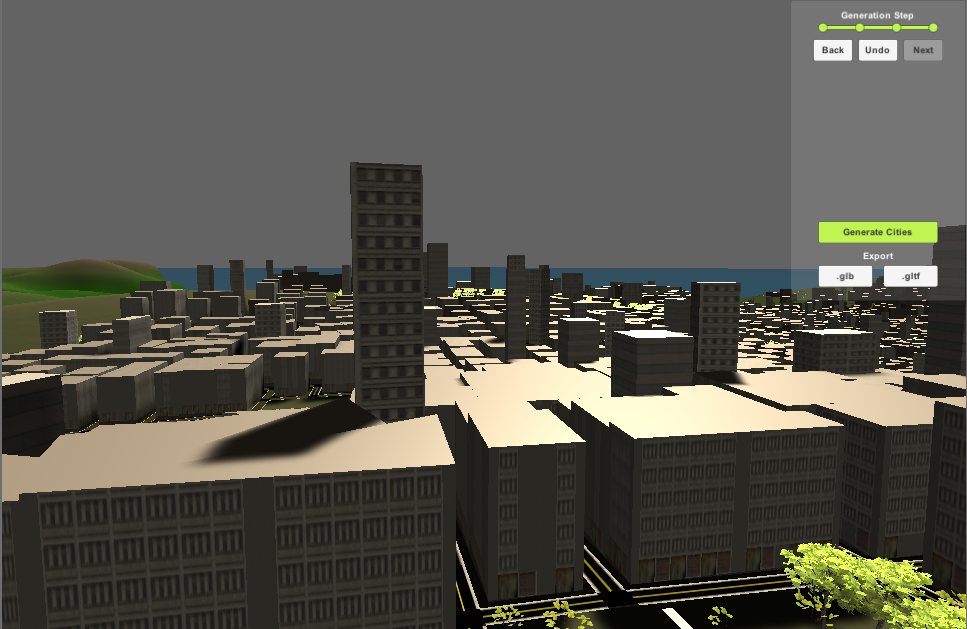
\includegraphics[width=0.7\textwidth]{figure/skyline.PNG}
  \caption{Skyline of \textit{Manhattan} and \textit{Skyscraper} buildings together, taller buildings being the skyscrapers}

  \label{fig:skyline-result}
\end{figure}

\textit{Manhattan} buildings are generated with stochastic L-systems, providing versatility via modular floor- and wall-type L-systems.
The final implementation had one floor-type and four wall-type generators, Figure \ref{fig:wall-segment-generator} shows examples of this in action.
\textit{FirstFloor} is the first floor type for every building, its wall segment generator produces a combination of shop windows, walls, and doors.
After the \textit{FirstFloor}, the floor-type generator repeats one of the following floor-type until the desired building height has been reached.
Note that each floor-type has its own wall segment generator that is run once per wall, and copied for each floor. 

\begin{itemize}
  \item \textit{NormalFloor} - generates wall and window segments, but it only generates half of the wall. For the other half, it copies the first half and reverses it. 
  \item \textit{EveryOtherFloor} - alternates between wall and window segments.
  \item \textit{RepeatWindowFloor} - only generates window segments.
\end{itemize}

Each of these strategies also start and end with a corner segment. 

\begin{figure}[H]
  \centering

  \begin{subfigure}[b]{0.3\textwidth}
    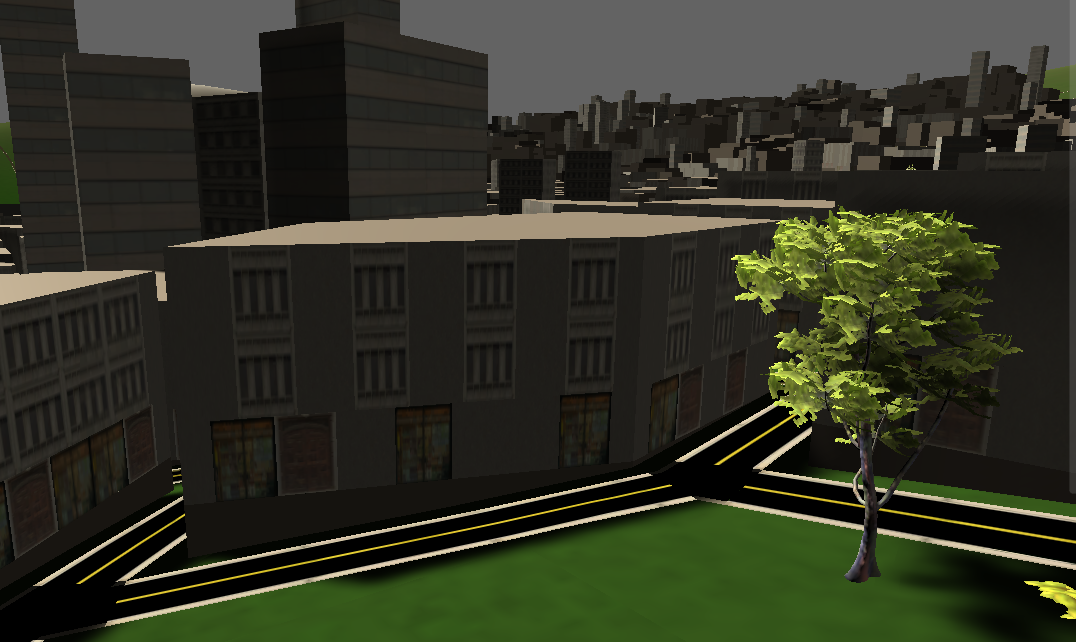
\includegraphics[width=\textwidth]{figure/building-every-other.PNG}
    \caption{\textit{EveryOtherFloor}.}
  \end{subfigure}
  \quad
  \begin{subfigure}[b]{0.3\textwidth}
    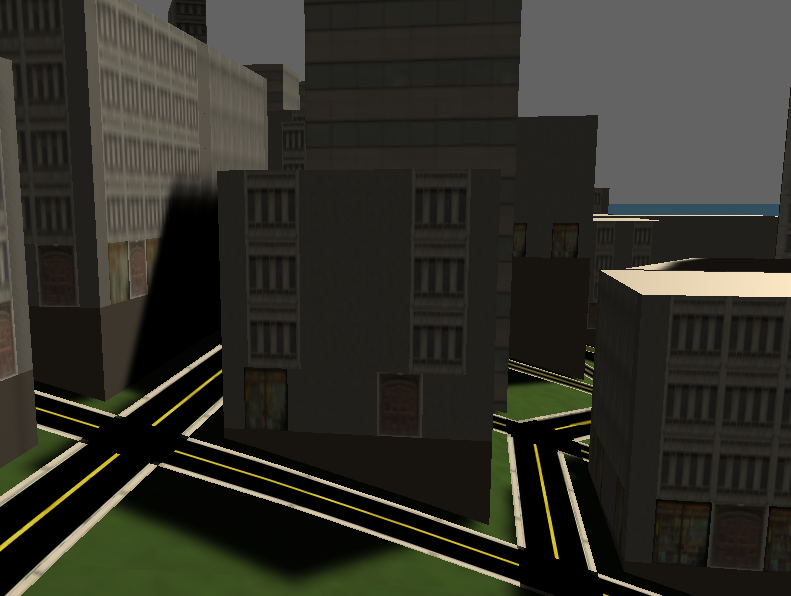
\includegraphics[width=\textwidth]{figure/building-normal.PNG}
    \caption{\textit{NormalFloor}.}
  \end{subfigure}
  \quad
  \begin{subfigure}[b]{0.3\textwidth}
      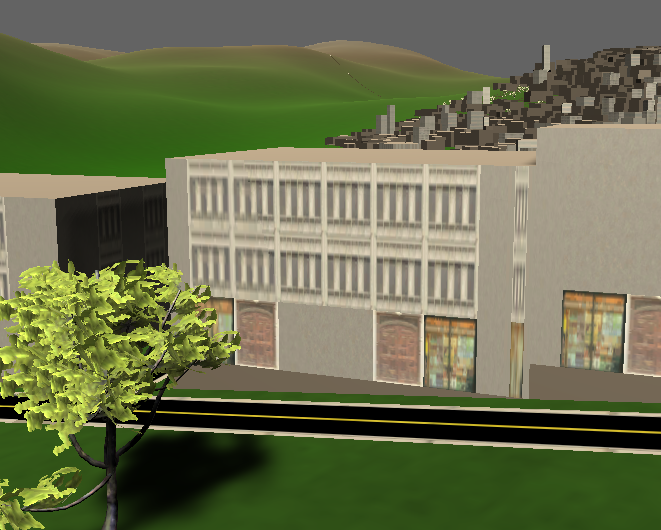
\includegraphics[width=\textwidth]{figure/building-only-window.PNG}
      \caption{\textit{RepeatWindowFloor}.}
  \end{subfigure}
  
  \caption{The three different wall segment generators. Notice that each building has a \textit{FirstFloor} wall segment generator on the first floor.}
  \label{fig:wall-segment-generator}
\end{figure}

The other building type is \textit{Skyscraper}, of which examples are shown in Figure \ref{fig:skyscraper-result}.
These buildings use texture atlases of windows from which different sub-regions are sampled to produce a procedural pattern of random windows.

\begin{figure}[H]
  \centering

  \begin{subfigure}[b]{0.45\textwidth}
    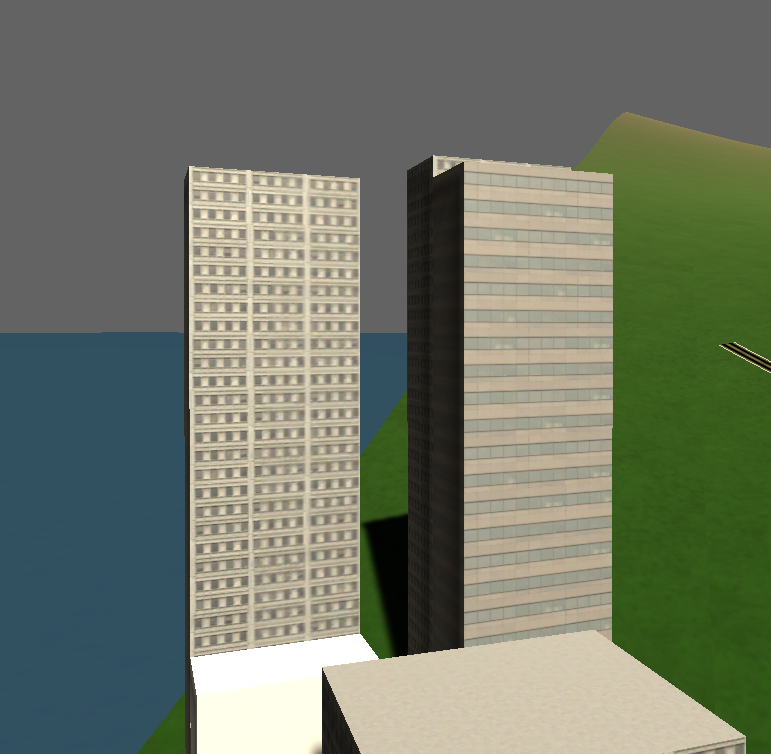
\includegraphics[width=\textwidth]{figure/skyscraper-close-up.PNG}
  \end{subfigure}
  \quad
  \begin{subfigure}[b]{0.45\textwidth}
    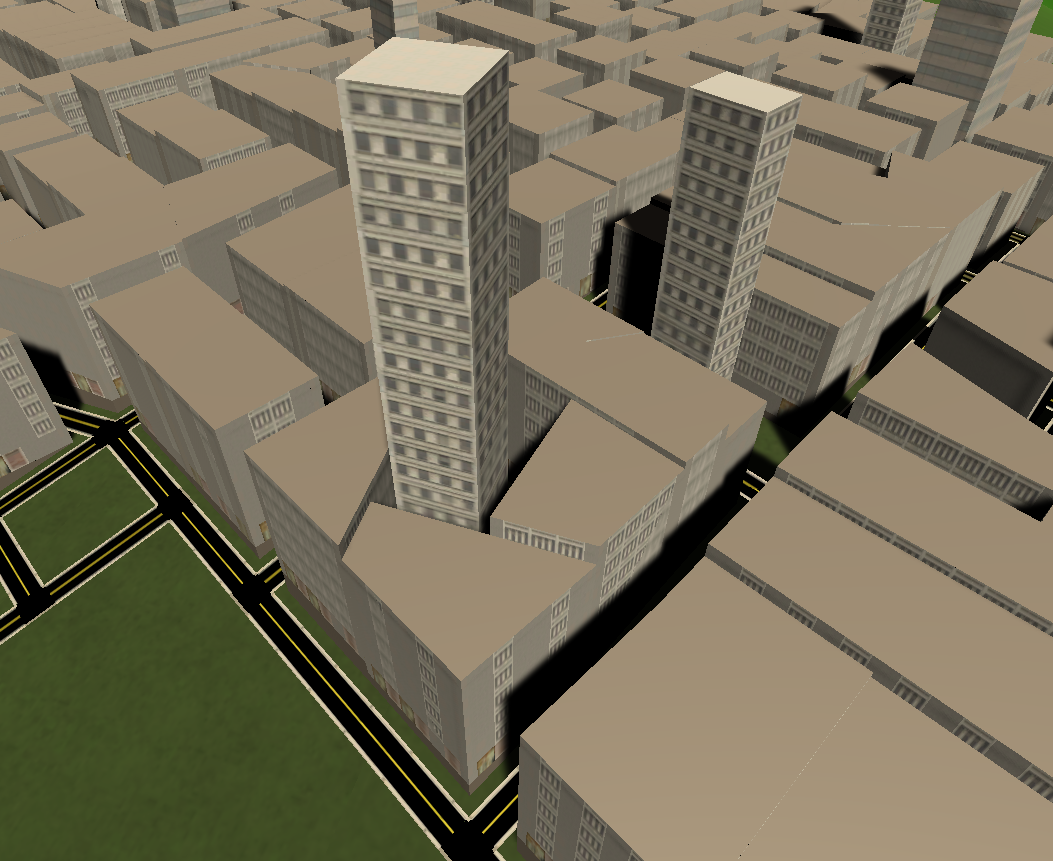
\includegraphics[width=\textwidth]{figure/wack.PNG}
  \end{subfigure}

  \caption{Two examples of skyscrapers generated in a city.}
  \label{fig:skyscraper-result}
\end{figure}
